\subsection{Уравнение состояния идеального газа. Изопроцессы}

Состояние данной массы газа полностью определено, если известны его давление, температура и объем. 
Эти величины называют параметрами состояния газа. Уравнение, связывающее параметры состояния, 
называют уравнением состояния.

\begin{definition}
    Для произвольной массы газа состояние газа описывается уравнением Менделеева—Клапейрона:
\end{definition}

$$pV = \frac{m}{\mu}RT$$

, где $p$ - давление, $V$ - объём, $m$ - масса, $M$ - молярная масса, $R$ - универсальная 
газовая постоянная ($R = 8,31 \frac{Дж}{моль \cdot К}$). Физический смысл универсальной газовой постоянной 
в том, что она показывает, какую работу совершает один моль идеального газа при изобарном расширении 
при нагревании на 1 К.

Уравнение Менделеева—Клапейрона показывает, что возможно одновременное изменение трех параметров, 
характеризующих состояние идеального газа. Однако многие процессы в газах, происходящие в природе и 
осуществляемые в технике, можно рассматривать приближенно как процессы, в которых изменяются лишь два 
параметра. Особую роль в физике и технике играют три процесса: изотермический, изохорный и изобарный.

\begin{definition}
    Изопроцессом называют процесс, происходящий с постоянной массой газа при одном постоянном параметре — температуре, давлении или объеме.
    Из уравнения состояния как частные случаи получаются законы для изопроцессов.
\end{definition}


\begin{definition}
    Изотермическим называют процесс, протекающий при постоянной температуре: $T = const$.
    Он описывается законом Бойля—Мариотта: $pV = const$.
\end{definition}

\begin{definition}
    Изохорным называют процесс, протекающий при постоянном объеме: $V = const$. 
    Для него справедлив закон Шарля: $\frac{p}{T} = const$.
\end{definition}

\begin{definition}
    Изобарным называют процесс, протекающий при постоянном давлении. 
    Уравнение этого процесса имеет вид $\frac{V}{T} = const$ при $p = const$ и называется законом Гей-Люссака.
\end{definition}

\begin{figure}[h]
    \centering
    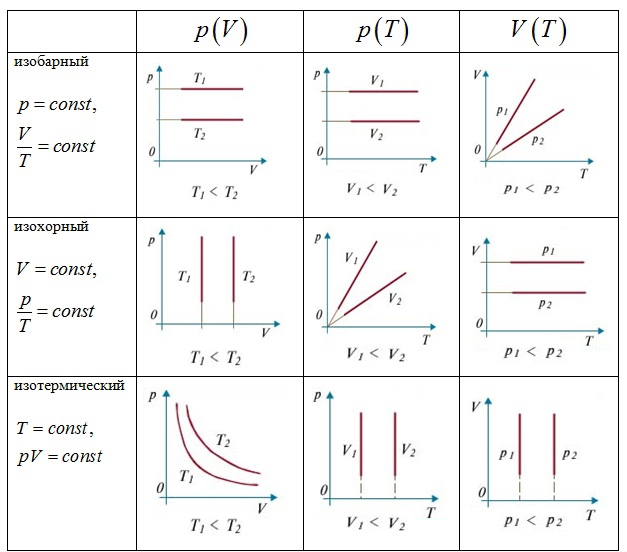
\includegraphics[width=0.4\linewidth]{imgs/q13i1.jpg}
\end{figure}

*Примечание: можно посмотреть МКТ*
